\documentclass[11pt]{article}
\usepackage[a4paper, margin=0.9in]{geometry}
\usepackage{amsmath}
\usepackage{booktabs}
\usepackage{float}
\usepackage{enumitem}
\usepackage{tikz}
\usetikzlibrary{positioning, arrows.meta}
\usepackage[hidelinks]{hyperref}
\setlength{\parskip}{3pt}

% ---- 3B results ----
% when the 3B runs are done: fill the numbers below and change \threeBtrue to \threeBtrue
\newif\ifthreeB
\threeBtrue
\newcommand{\mbppAcc}{0.84}
\newcommand{\mbppCI}{0.70}
\newcommand{\mbppQ}{0.56}
\newcommand{\mbppTok}{3076}
\newcommand{\plusAcc}{0.88}
\newcommand{\plusCI}{0.75}
\newcommand{\plusQ}{0.56}
\newcommand{\plusTok}{2994}
% --------------------

\title{Interactive Code Generation through Clarification:\\ Asking the Right Questions Before Writing Code}
\author{MADHAV SHAHI \\ IITG.AI, Phase 1 Project}
\date{September 2026}

\begin{document}
\maketitle

\begin{abstract}
\noindent
When a coding question is not clear, a language model usually guesses what the user wants. If the guess is wrong, the code is wrong. In this project, the model first asks a few yes/no questions in the form of unit tests, and only then gives its final code. The answers come from an oracle that runs each test on the reference solution. The questions are chosen using Expected Information Gain (EIG), following ``20 Questions for Code'' \cite{garg}. On the first 25 MBPP problems with Qwen2.5-Coder-1.5B, pass@1 went from 0.68 (one-shot) to 0.80, using about 15 times more tokens. With the 3B model, EIG reached 0.84 on MBPP and 0.88 on MBPP+. Because only 25 problems were used, the confidence intervals are wide and overlap, so this gain is promising but not yet proven. The paper \cite{garg} reports that a small model with EIG came close to a much larger model while using about 5 times fewer tokens, and lowering LLM cost in such ways is an active research topic \cite{frugal}.
\end{abstract}

\section{Introduction and Main Idea}
If you tell a tailor ``make me a shirt'', a good tailor first asks: what size, full or half sleeve, which colour. A bad tailor guesses. Code models often act like the bad tailor. For ``remove duplicate names from a list'', should ``Bob'' and ``bob'' count as the same? The prompt does not say, so the model picks one meaning.

My system makes the model act like the good tailor, using the idea of the game 20 Questions: a good question is one where any answer removes about half of the options. The model writes many possible programs, then asks a test where these programs disagree. Whatever the answer, many wrong programs get removed. EIG is a number that measures how good such a question is. I reimplemented the method of Garg, Kim and Xi \cite{garg}, a project from Stanford's CS224N course \cite{cs224n}, with smaller models on a free Colab GPU, and compared it with normal one-shot generation. Figure~\ref{fig:loop} shows the full loop.

\begin{figure}[H]
\centering
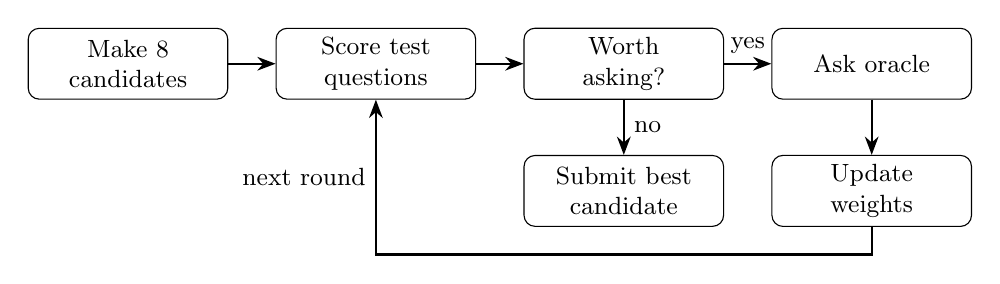
\begin{tikzpicture}[
  box/.style={draw, rounded corners, align=center, minimum height=0.9cm, text width=2.3cm, font=\small},
  arr/.style={-{Stealth}, thick}]
\node[box] (cand) {Make 8\\candidates};
\node[box, right=0.6cm of cand] (score) {Score test\\questions};
\node[box, right=0.6cm of score] (ask) {Worth\\asking?};
\node[box, right=0.6cm of ask] (oracle) {Ask oracle};
\node[box, below=0.7cm of oracle] (update) {Update\\weights};
\node[box, below=0.7cm of ask] (submit) {Submit best\\candidate};
\draw[arr] (cand) -- (score);
\draw[arr] (score) -- (ask);
\draw[arr] (ask) -- node[above, font=\small] {yes} (oracle);
\draw[arr] (oracle) -- (update);
\draw[arr] (ask) -- node[right, font=\small] {no} (submit);
\draw[arr] (update.south) -- ++(0,-0.35) -| node[pos=0.75, left, font=\small] {next round} (score.south);
\end{tikzpicture}
\caption{The ask-or-submit loop. It repeats until asking is not worth it or 4 questions are asked.}
\label{fig:loop}
\end{figure}

\section{Method}
\textbf{Candidates.} The model writes 8 programs per problem. To get more variety, half of them are told to try a different reasonable meaning of the problem. I remove candidates that do not define the needed function, have syntax errors, or fail the example test shown in the prompt. Duplicates are merged and get more weight.

\textbf{Questions.} The model writes tests like \texttt{assert f(x) == y}. A question is answered by running it on the reference solution, which says only yes or no.

\textbf{Scoring.} Each candidate $c_j$ has a weight $w_j$. Let $f_t(c_j)$ be 1 if it passes test $t$, 0 if it fails, and $\bot$ if it crashes. The weighted chance of passing is
\[
p_t = \frac{\sum_j w_j \mathbf{1}[f_t(c_j)=1]}{\sum_j w_j \mathbf{1}[f_t(c_j)\neq\bot]}, \qquad
\text{EIG}(t) = H_b\big(\epsilon + (1-2\epsilon)p_t\big) - H_b(\epsilon),
\]
where $H_b$ is binary entropy and $\epsilon$ is a small chance that the answer is wrong. As in the paper, the final score is
\[
\text{score}(t) = \text{EIG}(t)\cdot w_{\text{def}}(t)\cdot\big[(1-\lambda)+4\lambda p_t(1-p_t)\big]\cdot(1-\rho u_t),
\]
where $w_{\text{def}}$ is the weight of candidates that did not crash and $u_t$ the weight of those that did. Tests that crash on over half the weight, or where all working candidates agree, are skipped.

\textit{Example:} take 2 candidates with weight 0.5 each, where one passes a test and the other fails. Then $p_t = 0.5$ and $\text{EIG} = H_b(0.5) - H_b(0.02) = 1 - 0.14 = 0.86$. Nothing crashed, so the other factors are 1 and the score is 0.86. If both passed, $p_t = 1$ and the score would be 0, because the answer would tell us nothing.

\textbf{Update.} After an answer, agreeing candidates are multiplied by $1-\epsilon$, disagreeing ones by $\epsilon$, and crashed ones by $\eta$. Nothing is deleted fully, so one noisy answer cannot remove a good candidate forever.

\textbf{Ask or submit.} The system asks only if $\gamma \cdot p_{\text{next}} > p_{\text{now}}$, where $p_{\text{now}}$ is the highest weight now and $p_{\text{next}}$ the expected highest weight after the answer. The final answer is the candidate with the highest weight.

\textbf{Baseline.} One-shot uses the same model and prompt, writes one greedy answer and asks nothing.

\section{Setup}
Models: Qwen2.5-Coder-1.5B-Instruct and 3B-Instruct \cite{qwen}. Data: the first 25 problems of the MBPP sanitized test split \cite{mbpp} and of MBPP+ \cite{evalplus}, which has many more hidden tests. The prompt has the description, the function signature and the first test. Settings: 8 candidates, 8 tests per round, at most 4 questions, $\epsilon=0.02$, $\gamma=0.85$ as in the paper; $\eta=\lambda=\rho=0.5$ since the paper does not give them. I did not tune these three values, so checking how they change the results is future work. The paper uses 16 candidates; I used 8 because of limited free GPU time, but in the future I plan to use 16. Hardware: Colab T4 GPU, Kaggle T4 GPU,any GPU contained system. I report pass@1 (the share of problems where the final code passes all hidden tests) with the lower end of its 95\% confidence interval, the average number of questions and the average number of tokens. For code, pass@1 is the standard measure, and the paper \cite{garg} also uses it as its main metric.

\section{Results}
All results use only 25 problems per dataset, so every number has a wide confidence interval.

\begin{table}[H]
\centering
\small
\begin{tabular}{llcccc}
\toprule
Model & Method & pass@1 & Lower bound & Avg. questions & Avg. tokens \\
\midrule
1.5B & One-shot (MBPP) & 0.68 & 0.50 & 0.00 & 171 \\
1.5B & EIG (MBPP)      & 0.80 & 0.64 & 0.60 & 2628 \\
\ifthreeB
\midrule
3B   & EIG (MBPP)      & \mbppAcc & \mbppCI & \mbppQ & \mbppTok \\
3B   & EIG (MBPP+)     & \plusAcc & \plusCI & \plusQ & \plusTok \\
\fi
\bottomrule
\end{tabular}
\caption{Results on the first 25 problems of each dataset. ``Lower bound'' is the lower end of the 95\% confidence interval of pass@1.}
\end{table}

\textbf{One-shot vs EIG (1.5B).} On the same 25 problems, EIG solved 3 problems that one-shot failed and did not break any that one-shot solved. As a check, one-shot on the first 100 problems got 0.69, very close to the 69.2 the Qwen team reports , so my evaluation works correctly. The cost is about 15 times more tokens. On 13 problems the candidates already agreed, so EIG asked nothing, and all 13 passed. All 5 failures came from problems where it did ask, which are the harder or less clear ones.

\textbf{Examples.} In task 14 (volume of a triangular prism), one-shot wrote \texttt{l*b*h}, the volume of a box. After asking, EIG chose \texttt{(l*b/2)*h}, which is correct. This is the same kind of success case shown in the paper. In task 72, one-shot returned \texttt{n\%4 != 0} and EIG chose the correct \texttt{n\%4 != 2}. Task 20 (Woodall numbers) failed with both 1.5B methods, because no 1.5B candidate knew the formula. EIG can only pick from the candidates it has. The 3B model did solve it, which shows that better candidates matter.

\ifthreeB
\textbf{3B model.} I did not run one-shot with 3B, so these rows show how EIG does with a bigger model, not a gain over one-shot. On the same 25 MBPP problems, EIG with 3B got 0.84 against 0.80 with 1.5B: it solved 3 problems the smaller model missed and missed 2 that it solved. MBPP+ scored higher (0.88) even though its tests are stronger. This is because the first 25 MBPP+ problems are not the same set: 7 of them (tasks 2 to 9) are not in my MBPP list and are easy ones, and 6 of these 7 passed. On the 18 problems that are in both lists, EIG with 3B passed 16 on MBPP and also 16 on MBPP+, so the extra MBPP+ tests did not catch any new mistakes.
\else
\textbf{3B model.} Runs of EIG with Qwen2.5-Coder-3B on MBPP and MBPP+ are still in progress, and their results will be added to the repository.
\fi

\section{Problems I Faced and How I Solved Them}
\begin{itemize}[leftmargin=*, itemsep=2pt]
\item \textbf{Prompt cutoff:} EIG almost never asked, because the prompt for writing tests was cut off and the model gave few usable tests. \textbf{Fix:} completed the prompt and asked for only assert lines.
\item \textbf{Wrong function name:} for tests like \texttt{assert set(f(x)) == ...}, my code picked \texttt{set}. \textbf{Fix:} took the names from the reference code and picked the one used in the test.
\item \textbf{Messy test lines:} lines came as ``\texttt{1. assert}'', with backticks, or half written. \textbf{Fix:} cleaned each line and kept only valid Python.
\item \textbf{Similar candidates:} the candidates were almost the same, so there was nothing to ask. \textbf{Fix:} half of them try another meaning, with a higher temperature.
\item \textbf{Bad candidates:} broken code, duplicates, extra \texttt{print}/\texttt{assert} lines and infinite loops. \textbf{Fix:} filtered and merged candidates, removed extra lines, and ran code in a separate process with a time limit.
\item \textbf{Fair comparison:} \textbf{Fix:} used the same model, prompt, problems and seed for both methods.
\end{itemize}

\section{Limitations and Conclusion}
I used only 25 problems, so the gain is promising but not proven. I used small models and 8 candidates, and when no candidate is correct, questions cannot help. MBPP prompts are mostly clear, while the paper gets its biggest gains on prompts made unclear on purpose. I also did not compare against a larger one-shot model myself, so the cost claim relies on the paper. Next steps are running more problems, testing unclear prompts, and comparing with a larger model at the same token budget.

Still, asking a few good questions helped a small model: pass@1 went from 0.68 to 0.80 and no solved problem was lost. Like the good tailor, the model does better when it asks before it starts cutting.

\noindent Code: \url{https://github.com/Itsofficiallymadhav/NLP_Clarification/tree/eig-generated-tests}

\begin{thebibliography}{9}
\small
\bibitem{garg} R. Garg, A. Kim, J. Xi. \textit{20 Questions for Code: Improving Code Generation with Information-Theoretic Clarification}. Stanford CS224N Custom Project.
\bibitem{cs224n} C. Manning. \textit{CS224N: Natural Language Processing with Deep Learning}. Stanford University. \url{https://web.stanford.edu/class/cs224n/}
\bibitem{frugal} L. Chen, M. Zaharia, J. Zou. \textit{FrugalGPT: How to Use Large Language Models While Reducing Cost and Improving Performance}. 2023.
\end{thebibliography}

\end{document}